\documentclass[conference]{IEEEtran}

\usepackage[T1]{fontenc}
\usepackage[utf8]{inputenc}

\usepackage{cite}
\usepackage{url}
\usepackage{amsmath}
\usepackage{tabularx}
\usepackage{booktabs}
\usepackage{makecell}
\usepackage{array}
\usepackage{graphicx}
\usepackage{microtype}
\newcolumntype{Y}{>{\raggedright\arraybackslash}X}


\title{Chain Reaction: LLM-Guided Validation of Kubernetes Attack Chains}

\author{
\IEEEauthorblockN{Ashwin Charathsandran}
\IEEEauthorblockA{
FSCT-8611 Graduation Project\\
British Columbia Institute of Technology (BCIT)\\
Vancouver, BC, Canada\\
acharathsandran1@my.bcit.ca
}
}

\begin{document}
\maketitle

\begin{abstract}
Kubernetes security assessments commonly emphasize static configuration scanning and attack-path modeling to prioritize risk. While these techniques identify potentially dangerous conditions, they often fail to demonstrate what is actually exploitable from an in-cluster foothold under runtime constraints. Consequently, defenders may face many plausible multi-step paths with limited evidence indicating which chains can be executed in practice.

This project introduces \emph{Chain Reaction}, a Go-based in-cluster agent designed to run as a standard Kubernetes Pod. The agent operates solely with its assigned ServiceAccount credentials and ordinary cluster networking, assuming no node access and no out-of-band secrets. Chain Reaction targets multi-step attack chains spanning RBAC permissions, secret access, network pivots, and takeover preconditions. A chain step is considered validated only when the agent can execute the step from within the Pod using bounded probes and Kubernetes API interactions, and can capture supporting artifacts. Steps that cannot be executed are explicitly classified with failure reasons such as RBAC denial, unreachable network targets, guardrail enforcement, or missing prerequisites.

To drive efficient exploration, the system uses an LLM-guided, tool-oriented loop to enumerate relevant cluster objects, summarize effective permissions, test reachability, and validate steps incrementally while enforcing safety guardrails. Guardrails include allow-lists, rate limits, a time budget, and stop conditions to constrain both impact and cost.

The primary output is an evidence-backed, phase-labeled attack graph in which each node/edge is annotated with a phase and supported by collected artifacts, paired with an evidence bundle containing raw API responses, probe outputs, timestamps, and object snapshots. Graph edges are labeled as validated or theoretical based on direct runtime evidence. Evaluation on Kubernetes Goat (KG-001 through KG-005) used five repeated LLM-guided runs per batch. Scenario coverage rose from a mean of 0.88 (CV 12.45\%) on the initial pinned batch to 1.00 (CV 0.00\%) after a KG-004 probe fix and a KG-005 early-stop guard. Per-family reliability on the final guard-verify batch was 5/5 for every in-scope family. A one-sample Wilcoxon signed-rank test of that batch against the 0.80 target yields an exact two-sided $p=0.0625$, so $n=5$ cannot reject $H_0$ at $\alpha=0.05$ even when every run meets the target.
\end{abstract}

\begin{IEEEkeywords}
Kubernetes, assumed breach, attack-chain validation, RBAC, evidence logging
\end{IEEEkeywords}

\section{Introduction}

\subsection{Background and Motivation}
Kubernetes security has become harder to manage as clusters grow more complex. Access is controlled through identity and role-based access control (RBAC) rather than traditional network perimeters, workloads are short-lived, and policies are layered across multiple levels. Security scanners and posture management tools can flag possible risks, but they usually stop at listing theoretical attack paths. They do not test whether those paths actually work when runtime controls like NetworkPolicies, admission controllers, or missing Linux capabilities are in place.

This gap matters because defenders end up prioritizing risk based on what \emph{could} happen rather than what \emph{does} happen. A path that looks dangerous on paper might silently fail at the second or third step because of a policy that blocks network traffic or an RBAC rule that denies access. Without something that tests each step from inside the cluster, there is no reliable way to separate real risk from noise.

\section{Background and Literature Review}

Cloud-native security research has changed a lot in the last few years. Instead of only listing possible vulnerabilities, newer work is moving toward tools that can actively test whether an attack is doable in a real environment. This shift matters because Kubernetes clusters are complex: traditional network boundaries are less important, access is mostly controlled through identity, role-based access control (RBAC), and container permissions, and an attack path that looks possible on paper often requires multiple steps. In practice, these chains can fail because of runtime controls such as NetworkPolicies, admission controllers, or missing Linux capabilities.

This literature review summarizes recent work across five themes that relate to validating Kubernetes attack chains. Based on 20 recent academic papers and representative commercial tools, it highlights gaps in current methods and explains why \emph{Chain Reaction} is needed. \emph{Chain Reaction} is designed to run inside a cluster, execute multi-step Kubernetes attack chains from an assumed-breach position, and collect evidence that each step truly worked.

\subsection{Kubernetes Security Background}
Kubernetes clusters are controlled through a small set of primitives that shape how attackers move. The control plane centers on the API server (the request gateway), etcd (the persistent state store), and per-node kubelets that enforce Pod specs and expose node-level management interfaces. The API server mediates access to cluster state, and workloads interact with it primarily through credentials rather than a traditional network perimeter. In most deployments, Pods authenticate to the API using ServiceAccount tokens that are mounted into the container filesystem by default. RBAC objects (Roles/RoleBindings and ClusterRoles/ClusterRoleBindings) bind those identities to verbs and resources, defining what an in-cluster foothold can read or modify.

Runtime controls often make the difference between a theoretical path and an executable chain. NetworkPolicies can prevent lateral movement even when Services and Endpoints exist; admission controllers and policy engines can block privileged Pods or unsafe fields; and Linux capabilities, seccomp, and container runtime isolation can prevent container-level escalation techniques. As a result, an attack edge that looks reachable via configuration analysis may fail at runtime because a required permission, network route, or runtime privilege is absent. This paper focuses on validating those chains under runtime constraints from an assumed-breach Pod perspective.

\subsection{Theme 1: LLM-Driven Autonomous Offensive Security}
Large Language Models (LLMs) are increasingly being used to support offensive security. Recent systems show that an agent can plan a multi-step attack, take actions, observe results, and adjust as it goes. However, most evaluations are still based on traditional environments like Linux hosts or web applications. They do not fully cover Kubernetes-specific privilege building blocks such as ServiceAccounts, ConfigMaps, and cluster-scoped RBAC. Table \ref{tab:litmatrix-theme1} summarizes key work in this area.

\begin{table*}[t!]
\centering
\caption{Theme 1: LLM-Driven Autonomous Offensive Security}
\label{tab:litmatrix-theme1}
\scriptsize
\setlength{\tabcolsep}{5pt}
\renewcommand{\arraystretch}{1.3}
\begin{tabularx}{\textwidth}{l p{2.6cm} X X}
\toprule
\textbf{Author \& Year} & \textbf{Method} & \textbf{Key Findings} & \textbf{Gap vs. Proposal} \\
\midrule
\textbf{Deng et al., 2024} \cite{deng2024pentestgpt} & Hybrid (System Design + Benchmark) & Shows that an LLM can guide multi-step penetration testing using a tool-calling architecture. Supports a basic plan-act-observe loop. & Still depends heavily on a human for execution steps and focuses on standard OS and web targets, not Kubernetes. \\
\addlinespace
\textbf{Fang et al., 2024} \cite{fang2024llm} & Quantitative (Agent eval on 15 CVEs) & Demonstrates that GPT-4 style agents can exploit many 1-day vulnerabilities when given CVE descriptions. & Focuses on single CVEs, not multi-step Kubernetes privilege escalation chains across real cluster configurations. \\
\addlinespace
\textbf{Xu et al., 2024} \cite{xu2024autoattacker} & Hybrid (Multi-agent system design) & Uses separate agents (summarizer, planner, navigator) to manage longer post-breach workflows. & Evaluations assume traditional networks and do not model Kubernetes-native privileges like ServiceAccounts, ConfigMaps, and RBAC. \\
\addlinespace
\textbf{Happe \& Cito, 2023} \cite{happe2023llms} & Quantitative (Priv-esc scenarios) & Benchmarks how well LLMs handle Linux privilege escalation tasks across different scenario difficulties. & Does not capture the distributed nature of Kubernetes, where privilege escalation often involves pivoting between pods, nodes, and APIs. \\
\addlinespace
\textbf{Shen et al., 2024} \cite{chen2024pentestagent} & Hybrid (Multi-agent system) & Splits tasks into recon, exploit, and reporting agents to improve performance over long runs. & Targets enterprise infrastructure more than Kubernetes and does not assume an in-cluster identity model. \\
\addlinespace
\textbf{Happe et al., 2025} \cite{happe2025benchmarking} & Survey and Meta-analysis & Finds that benchmarking in LLM offensive security is often not reproducible across platforms. & Reinforces a gap that \emph{Chain Reaction} addresses by using a standardized baseline environment (Kubernetes Goat). \\
\addlinespace
\textbf{Isozaki et al., 2024} \cite{isamu2024towards} & Hybrid (Benchmark Design) & Proposes a standardized benchmark for testing LLM penetration tools across phases like enumeration and exploitation. & Notes the need for more reproducible evaluation setups, including cloud-native contexts, but does not focus on Kubernetes chain execution. \\
\bottomrule
\end{tabularx}
\end{table*}

\subsection{Theme 2: Attack Graph Modeling and Generation}
Attack graphs are widely used to represent possible lateral movement and privilege escalation paths. Generating these graphs from configuration data is a well-studied problem. The main limitation in cloud-native environments is that the edges in the graph usually represent \emph{possibility}, not confirmed exploitability. In Kubernetes, a graph may indicate an attacker can move from one pod to another, but runtime controls can quietly block the step. What is missing is an execution engine that can test a path from an assumed-breach pod and confirm what is actually reachable. Table \ref{tab:litmatrix-theme2} outlines foundational work in this area.

\begin{table*}[t!]
\centering
\caption{Theme 2: Attack Graph Modeling, Generation, and Analysis}
\label{tab:litmatrix-theme2}
\scriptsize
\setlength{\tabcolsep}{5pt}
\renewcommand{\arraystretch}{1.3}
\begin{tabularx}{\textwidth}{l p{2.6cm} X X}
\toprule
\textbf{Author \& Year} & \textbf{Method} & \textbf{Key Findings} & \textbf{Gap vs. Proposal} \\
\midrule
\textbf{Ou et al., 2006} \cite{ou2006scalable} & Algorithmic Logic Programming & Uses Datalog-based reasoning over configuration and vulnerabilities to generate scalable attack graphs. & Predates Kubernetes and does not validate edges at runtime. Paths remain theoretical. \\
\addlinespace
\textbf{Li et al., 2022} \cite{ibrahim2022strategies} & Survey and Hybrid Framework & Surveys modular approaches that separate topology, vulnerability data, and analysis layers to scale attack graphs. & Focuses on enterprise networks and does not provide live execution or proof actions. \\
\addlinespace
\textbf{Palma \& Angelini, 2023} \cite{bernieri2023scalable} & Modular Framework Design & Proposes an analysis-driven approach that scales to large environments. & Does not account for Kubernetes churn and short-lived workloads. \\
\addlinespace
\textbf{Tayouri et al., 2025} \cite{ditizio2024coral} & Logical attack graphs with incremental updates & Builds container-focused logical attack graphs that update as pods and containers change. & Models what \emph{could} happen based on RBAC and network state but does not validate reachability through execution. \\
\addlinespace
\textbf{Mensah, 2019} \cite{sultan2019generation} & Cloud Topology Retrieval & Studies dynamic attack graph updates by tracking changing IaaS state in cloud providers. & Targets IaaS more than Kubernetes API resources and RBAC-driven permissions. \\
\addlinespace
\textbf{Smiliotopoulos et al., 2024} \cite{sultan2024detecting} & Systematic Survey & Shows configuration paths often fail at runtime because of policies and missing capabilities. & Supports the need for active validation, but the work is detection-focused rather than execution-focused. \\
\bottomrule
\end{tabularx}
\end{table*}

\subsection{Theme 3: Container and Cloud-Native Threat Modeling}
Threat modeling work helps define what attackers might target in container systems. Using methods like STRIDE, researchers map threats across images, runtime behavior, orchestration, and networking. These taxonomies are useful because they describe the attack surface that an offensive agent should test. However, most of this work stays at the analysis level. It explains what threats exist but does not show how to autonomously confirm them inside a live cluster with real restrictions. Table \ref{tab:litmatrix-theme3} summarizes this theme.

\begin{table*}[t!]
\centering
\caption{Theme 3: Container and Cloud-Native Threat Modeling}
\label{tab:litmatrix-theme3}
\scriptsize
\setlength{\tabcolsep}{5pt}
\renewcommand{\arraystretch}{1.3}
\begin{tabularx}{\textwidth}{l p{2.6cm} X X}
\toprule
\textbf{Author \& Year} & \textbf{Method} & \textbf{Key Findings} & \textbf{Gap vs. Proposal} \\
\midrule
\textbf{Wong et al., 2021} \cite{getahun2021security} & STRIDE Methodology and Attack Analysis & Maps threats across image, runtime, orchestration, and networking layers and provides a clear taxonomy of container attack vectors. & Does not include a method for validating these threats under real cluster constraints. \\
\addlinespace
\textbf{Jarkas et al., 2025} \cite{lin2025container} & Systematic Survey & Reviews 200+ container vulnerabilities and groups them into many exploit categories. & Strong as a reference, but it does not provide in-cluster execution to test exploitability. \\
\bottomrule
\end{tabularx}
\end{table*}

\subsection{Theme 4: Adversary Emulation and Breach Simulation Frameworks}
Adversary emulation and Breach and Attack Simulation (BAS) tools are the closest match to what \emph{Chain Reaction} aims to do. Some frameworks also use planning methods to operate in partially observable environments. The main gap is where and how they run. Many systems execute procedures on endpoints (Windows or Linux) or in simulated networks. They usually do not run as a Kubernetes pod using real in-cluster credentials, and they often do not produce step-by-step, auditable evidence artifacts tied to Kubernetes actions. Table \ref{tab:litmatrix-theme4} compares major examples.

\begin{table*}[t!]
\centering
\caption{Theme 4: Adversary Emulation and Breach Simulation}
\label{tab:litmatrix-theme4}
\scriptsize
\setlength{\tabcolsep}{5pt}
\renewcommand{\arraystretch}{1.3}
\begin{tabularx}{\textwidth}{l p{2.6cm} X X}
\toprule
\textbf{Author \& Year} & \textbf{Method} & \textbf{Key Findings} & \textbf{Gap vs. Proposal} \\
\midrule
\textbf{Miller et al., 2018} \cite{miller2021automated} & AI Planning combined with Caldera & Uses planning approaches to adapt as new environment information is discovered. & Mostly assumes OS-level agents and does not focus on Kubernetes-native steps like ServiceAccount token use. \\
\addlinespace
\textbf{Microsoft Research, 2021} \cite{microsoft2021cyberbattlesim} & Reinforcement Learning Simulation Framework & Provides a platform for training autonomous attacker agents for lateral movement. & Primarily simulated and abstract, not executing real actions against live Kubernetes clusters. \\
\addlinespace
\textbf{Chang et al., 2025} \cite{applebaum2022characterizing} & Experimental Evaluation & Finds that Caldera covers many techniques but depends on traditional endpoints. & Does not operate as an in-cluster Kubernetes pod with native credentials and evidence bundles. \\
\addlinespace
\textbf{Hackl{\"a}nder-Jansen et al., 2025} \cite{lam2025autonomous} & Multi-agent LLM guided by ATT\&CK & Uses LLM planning to emulate multi-stage adversaries with broad technique coverage. & Evaluated in enterprise network settings and does not use a Kubernetes assumed-breach model. \\
\bottomrule
\end{tabularx}
\end{table*}

\subsection{Theme 5: Runtime Exploitability Validation}
The purpose of attack chain analysis is to separate theoretical risk from what an attacker can really do. Some research argues that an agent must actively probe its environment to confirm reachability and feasibility under partial observability. The missing piece is applying this idea cleanly inside Kubernetes, where proof actions must work through real API responses, RBAC enforcement, rate limits, and egress limits. Table \ref{tab:litmatrix-theme5} highlights this direction.

\begin{table*}[t!]
\centering
\caption{Theme 5: Runtime Exploitability Validation}
\label{tab:litmatrix-theme5}
\scriptsize
\setlength{\tabcolsep}{5pt}
\renewcommand{\arraystretch}{1.3}
\begin{tabularx}{\textwidth}{l p{2.6cm} X X}
\toprule
\textbf{Author \& Year} & \textbf{Method} & \textbf{Key Findings} & \textbf{Gap vs. Proposal} \\
\midrule
\textbf{Terranova et al., 2024} \cite{garcia2024deep} & Deep RL Agent Simulation & Shows that an agent probing its environment can discover attack paths under partial observability. & Results are based on simulation and do not address real Kubernetes constraints like API enforcement, rate limits, or restricted egress. \\
\bottomrule
\end{tabularx}
\end{table*}

\subsection{Competitive Landscape and Synthesis}
Commercial cloud-native security tools often focus on defense and posture management (for example, CNAPP products like Wiz and Orca). Autonomous pentesting platforms (for example, Horizon3.ai's NodeZero and Pentera) are closer to attack-chain execution because they safely run exploits and chain misconfigurations. However, their evidence guarantees, reasoning transparency, and decision logic are mostly proprietary and are not described at an academic level.

Across the five themes, three gaps show up consistently:
\begin{enumerate}
    \item \textbf{Few Kubernetes-native LLM agents:} Existing LLM attack agents usually focus on web apps or OS targets and do not specialize in Kubernetes primitives from an in-cluster identity.
    \item \textbf{Attack graphs stay theoretical:} Many systems can generate plausible paths, but they do not execute bounded proof actions to confirm whether edges are actually traversable.
    \item \textbf{Limited evidence-backed reporting:} Current approaches rarely produce phase-labeled graphs with clear, auditable evidence bundles that prove exploitability step by step.
\end{enumerate}

\emph{Chain Reaction} is designed to address these gaps by moving from theoretical correlation to runtime validation. Instead of assuming a path is reachable, it executes Kubernetes-native steps from an assumed-breach pod and produces artifacts that document what was verified inside the cluster.

\section{Research Problem and Objectives}
Current Kubernetes attack-path tools identify plausible multi-step chains but do not validate whether those chains can actually be executed from an in-cluster identity. The attack graphs they produce typically lack runtime evidence. To the best of our knowledge, existing open-source tools do not run from an assumed-breach Pod position to confirm step-by-step exploitability using safe, bounded probes while collecting auditable artifacts.

\subsection{Research Questions}
This project is guided by three research questions:
\begin{enumerate}
    \item \textbf{RQ1:} Can an LLM-guided agent running inside a Kubernetes pod validate multi-step attack chains by executing bounded proof actions against real cluster state?
    \item \textbf{RQ2:} What fraction of theoretically modeled attack paths in a controlled Kubernetes environment (Kubernetes Goat) can be confirmed as runtime-validated chains?
    \item \textbf{RQ3:} How do guardrail mechanisms (allow-lists, rate limits, time budgets, stop conditions) affect the balance between exploration coverage and operational safety?
\end{enumerate}

\subsection{Scope and Assumptions}
This work assumes an \emph{assumed-breach Pod} foothold: the agent runs as a standard Kubernetes Pod and operates using only its assigned ServiceAccount token and ordinary cluster networking. It assumes no node access, no privileged container execution, and no out-of-band secrets. The evaluation environment is bounded to Kubernetes Goat \cite{kubegoat2023} deployed in a reproducible local cluster, and the in-scope scenario families are KG-001 through KG-005. The system treats the LLM endpoint as untrusted input and enforces guardrails (namespace allow-lists, rate limits, time budgets, and stop conditions) to bound impact and execution cost.

\subsection{Relevance to Cybersecurity Practice}
For defenders, static attack graphs and scanner findings are difficult to prioritize when they cannot be replayed or audited. A runtime validator that produces timestamped, replayable artifacts can help incident responders and security engineers distinguish chains that are practically exploitable from those that are blocked by policy, identity scoping, or runtime controls. By tying each validated step to evidence, the approach aims to bridge theoretical modeling with defender workflows that require verification, repeatability, and clear failure reasons.

\section{Project Approach and Methodology}

\subsection{Overview}
Chain Reaction is a Go-based agent that runs as a normal Kubernetes Pod. It uses an LLM-guided, tool-calling loop to discover cluster objects, check permissions, test network reachability, and validate attack-chain steps one at a time. The agent only uses its assigned ServiceAccount credentials and ordinary cluster networking. It does not assume node access and does not rely on out-of-band secrets. The project follows four phases.

\subsection{Phase 1: Environment Setup and Baseline}
The test environment is Kubernetes Goat \cite{kubegoat2023}, a deliberately vulnerable Kubernetes cluster with a set of known misconfigurations and exploitable scenarios. Kubernetes Goat runs on a local kind cluster with Kubernetes 1.30. Before running the agent, each scenario is manually catalogued to build a ground-truth list of expected attack chains and the steps they involve. This catalogue becomes the baseline that all later measurements are compared against.

\subsection{Phase 2: Agent Architecture and Tool Implementation}
The agent follows a plan-act-observe loop. Each iteration, the LLM gets the current cluster context, which includes discovered objects, effective permissions, and prior step outcomes, and picks a tool to run. The core tools are:
\begin{itemize}
    \item \textbf{Kubernetes API Prober} - lists namespaces, pods, services, secrets, configmaps, roles, and bindings through \texttt{client-go}.
    \item \textbf{RBAC Analyzer} - checks what the agent's ServiceAccount can actually do by issuing \texttt{SelfSubjectAccessReview} and \texttt{SelfSubjectRulesReview} requests.
    \item \textbf{Network Reachability Checker} - tests TCP and HTTP connectivity to discovered service endpoints, the API server, and the kubelet from within the pod.
    \item \textbf{Secret Reader} - tries to retrieve secret objects to see if RBAC allows it.
    \item \textbf{Token Projector} - inspects mounted ServiceAccount tokens and tests their scope through API authentication checks.
\end{itemize}

Table \ref{tab:tool_suite} summarizes the tool suite and the evidence outputs each tool contributes to the final artifacts.

\begin{table*}[t!]
\centering
\caption{Core tool suite used in the ReAct loop and the evidence each tool emits.}
\label{tab:tool_suite}
\scriptsize
\setlength{\tabcolsep}{6pt}
\renewcommand{\arraystretch}{1.2}
\begin{tabularx}{\textwidth}{l l X}
\toprule
\textbf{Tool} & \textbf{Category} & \textbf{Primary outputs (evidence)} \\
\midrule
Kubernetes API Prober & Discovery & Object lists and snapshots (namespaces, pods, services, RBAC objects) used to build graph nodes \\
RBAC Analyzer & Introspection & Access-review responses proving allowed/denied verbs on resources; used to justify or refute privilege edges \\
Network Reachability Checker & Validation & TCP/HTTP probe results (success, timeout, refusal) with target endpoint metadata; used to validate lateral-movement edges \\
Secret Reader & Validation & Secret get/list responses (or explicit denials) with redaction as needed; used to validate credential-access edges \\
Token Projector & Validation & Token mount inspection and API authentication checks; used to validate assumed-breach identity scope \\
\bottomrule
\end{tabularx}
\end{table*}

Tools are read-only by default, with bounded, pre-approved exceptions only when a specific scenario validation requires them. Safety guardrails keep the agent bounded: an allow-list limits which namespaces and resource types are in scope, a per-step rate limiter caps API calls, a time budget kills the run after a set duration (default: 5 minutes), and stop conditions halt execution if the agent tries to do something that is not allowed.

\subsection{Phase 3: Chain Execution and Evidence Collection}
The agent walks each attack chain step by step. A step counts as \emph{validated} only when the agent can run the matching probe from inside the pod and capture a supporting artifact. Artifacts include things like raw API response bodies, TCP handshake results, decoded secret values, and permission check outputs. Steps that fail are tagged with a reason: RBAC denial, unreachable network target, missing prerequisite, or guardrail enforcement.

The main output is a phase-labeled attack graph where each node is a cluster object or identity and each edge is a validated or theoretical transition. Edges are annotated with the execution status and linked to an evidence bundle that holds timestamped API responses, probe outputs, and object snapshots.

\subsection{Phase 4: Evaluation and Analysis}
The agent runs across in-scope Kubernetes Goat scenarios. Each run produces a graph and evidence bundle. Metrics are collected automatically and aggregated across repeated runs. The evaluation compares what the agent validated against the manually built baseline and against a static analysis pass that lists theoretical paths without actually running anything.

\subsection{Measurement Models and Metrics}

The evaluation relies on four main metrics:

\begin{enumerate}
    \item \textbf{Scenario Coverage (SC):} The fraction of Kubernetes Goat scenarios where the agent validates at least one full attack chain. The target is $\text{SC} \geq 0.80$.
    \begin{equation}
        \text{SC} = \frac{|\{\text{scenarios with} \geq 1 \text{ validated chain}\}|}{|\{\text{total scenarios}\}|}
    \end{equation}

    \item \textbf{Step Validation Rate (SVR):} The fraction of theoretical chain steps from the baseline that the agent confirms as actually executable at runtime.
    \begin{equation}
        \text{SVR} = \frac{|\{\text{validated steps}\}|}{|\{\text{theoretical steps in baseline}\}|}
    \end{equation}

    \item \textbf{Time-to-Chain (TTC):} Wall-clock seconds from agent start to the first fully validated chain in a given scenario.

    \item \textbf{API Call Volume (ACV):} Total Kubernetes API requests the agent makes per scenario run. This measures efficiency and gives a rough sense of cost.
\end{enumerate}

Two additional metrics round out the picture:
\begin{itemize}
    \item \textbf{Run-to-Run Stability:} The coefficient of variation of SC and SVR across five repeated runs per scenario. This shows how consistent the LLM-guided exploration is from one run to the next.
    \item \textbf{Guardrail Trigger Rate:} The fraction of runs where at least one guardrail (rate limit, time budget, allow-list block) fires. This tells us whether the safety constraints are actually doing something or just sitting idle.
\end{itemize}

\subsection{Statistical and Research Methods}

This proposal uses a \textbf{quantitative}, controlled-benchmark evaluation design in a bounded lab environment. The independent variable is the validation approach (LLM-guided runtime validator vs. static/theoretical baseline), and the dependent variables are the metrics defined in the prior section (SC, SVR, TTC, ACV, stability, and guardrail trigger rate). This aligns with FSCT 8611's scope: design and proposal only, with implementation and measured results produced in FSCT 8622.

\subsubsection{Hypotheses}
The primary comparative hypothesis focuses on the gap between theoretical paths and runtime-validated steps (RQ2). Let $\Delta \text{SVR}_s$ be the per-scenario difference between the agent SVR and the static baseline SVR for scenario $s$.
\begin{itemize}
    \item \textbf{H0:} The median $\Delta \text{SVR}_s \leq 0$ (runtime validation does not improve step validation rate relative to static analysis).
    \item \textbf{H1:} The median $\Delta \text{SVR}_s > 0$ (runtime validation yields higher step validation rate than static analysis).
\end{itemize}
These hypotheses are evaluated using a paired Wilcoxon signed-rank test over scenarios at $\alpha = 0.05$.

\subsubsection{Research-Question Alignment}
Table \ref{tab:rq_alignment} summarizes how the evaluation design answers the three research questions.

\begin{table*}[t!]
\centering
\caption{Research questions aligned to measurements and analysis.}
\label{tab:rq_alignment}
\scriptsize
\setlength{\tabcolsep}{6pt}
\renewcommand{\arraystretch}{1.2}
\begin{tabularx}{\textwidth}{l X X}
\toprule
\textbf{RQ} & \textbf{Evidence/Measurement} & \textbf{Analysis} \\
\midrule
RQ1 & Existence of at least one fully validated multi-step chain from the assumed-breach Pod; evidence bundle links per step & Report scenario-level success (SC) and summarize common validated step patterns \\
RQ2 & Step-level gap between theoretical baseline steps and runtime-confirmed steps (SVR); edge outcomes and failure reasons & Compare SVR distributions vs. static baseline; paired Wilcoxon signed-rank test on per-scenario SVR \\
RQ3 & Guardrail triggers and exploration efficiency under different guardrail settings (strict vs. default vs. relaxed) & Compare SC/SVR/TTC/ACV and trigger rates across guardrail profiles; interpret tradeoffs between coverage and safety \\
\bottomrule
\end{tabularx}
\end{table*}

Because the LLM introduces randomness through its sampling process, each scenario is run five times. Basic descriptive statistics (mean, standard deviation, coefficient of variation) are computed for SC, SVR, TTC, and ACV across those runs.

The main statistical question is whether the agent's validated coverage is meaningfully better than what static analysis alone can produce. To test this, a paired Wilcoxon signed-rank test is used on the per-scenario SVR values for the agent versus the static baseline. This non-parametric test fits well here because sample sizes per scenario are small and the step-level outcomes are ordinal. The significance threshold is $\alpha = 0.05$.

Beyond that, Spearman's rank correlation is used to look at two relationships. First, whether higher API call volume actually leads to higher validation rates or just reflects the agent spinning its wheels. Second, whether time-to-chain grows with chain length (number of steps in the baseline chain), which would suggest the system scales predictably.

\subsection{Data Sources and Data Collection}

\subsubsection{Test Environment}
The main data source is Kubernetes Goat, an open-source, intentionally vulnerable Kubernetes deployment. It gives a reproducible set of misconfigured scenarios that cover things like RBAC over-provisioning, exposed secrets, container escapes, and network-level weaknesses. The cluster runs on kind (Kubernetes IN Docker) version 0.20+ with Kubernetes 1.30, using a single-node setup so the environment stays consistent between runs.

\subsubsection{Data Collected Per Run}
Each agent run produces four types of artifacts:
\begin{itemize}
    \item \textbf{Attack graph:} A JSON-serialized directed graph. Nodes are cluster objects or identities, and edges carry a validation status, phase label, and reference to the supporting evidence.
    \item \textbf{Evidence bundle:} A folder of timestamped files that includes raw API responses (JSON), TCP probe results, decoded secret values (redacted where needed), RBAC check outputs, and object snapshots.
    \item \textbf{Run log:} A structured log in JSON Lines format. It records each LLM prompt, tool call, tool response, decision rationale, and guardrail trigger event, all with timestamps.
    \item \textbf{Metric summary:} A JSON file with the computed values for SC, SVR, TTC, ACV, and guardrail events for that run.
\end{itemize}

Table \ref{tab:artifacts} summarizes the artifacts and their intended use as auditable evidence outputs.

\begin{table*}[t!]
\centering
\caption{Primary artifacts produced per scenario run (evidence-first outputs).}
\label{tab:artifacts}
\scriptsize
\setlength{\tabcolsep}{6pt}
\renewcommand{\arraystretch}{1.2}
\begin{tabularx}{\textwidth}{l l X}
\toprule
\textbf{Artifact} & \textbf{Format} & \textbf{Purpose / Key contents} \\
\midrule
Attack graph & JSON & Directed graph with nodes (resources/identities) and edges (transitions) labeled as validated/theoretical/failed; references evidence IDs \\
Evidence log & JSONL (hash-chained) & Append-only, timestamped event stream for tool calls, responses, guardrail decisions, and validation outcomes; supports offline auditing \\
Evidence bundle & Files (JSON/TXT) & Raw supporting artifacts (API response bodies, probe outputs, snapshots); organized per run with stable filenames \\
Metric summary & JSON & Scenario-level metrics (SC/SVR/TTC/ACV), run-to-run stability values, and guardrail trigger counts \\
\bottomrule
\end{tabularx}
\end{table*}

\subsubsection{Volume and Sampling}
With $N$ scenarios in Kubernetes Goat and 5 runs per scenario, the full dataset has $5N$ independent runs. No sampling is applied because every scenario is included. The manual baseline catalogue is built once and frozen before agent evaluation starts.

\subsection{Data Analysis Techniques}

\subsubsection{Tools and Software}
Analysis is done in the Chain Reaction Go pipeline (\texttt{chain-reaction analyze} and \texttt{compare}). Descriptive statistics, the Wilcoxon signed-rank test, Spearman correlation, SVG figures, Markdown tables, and HTML reports are generated offline from frozen \texttt{validation-metrics.json} artifacts without a live cluster.

\subsubsection{Analysis Pipeline}
The analysis happens in three stages:
\begin{enumerate}
    \item \textbf{Metric extraction:} Run logs and metric summaries are parsed into a single dataframe indexed by scenario and run number. Attack graphs are loaded into \texttt{networkx} so we can look at things like node count, edge count, connected components, and the fraction of edges that are validated.
    \item \textbf{Descriptive analysis:} Per-scenario distributions of SC, SVR, TTC, and ACV are computed and shown through box plots and bar charts. Heatmaps display step validation outcomes for each scenario across all five runs.
    \item \textbf{Comparative analysis:} The agent's SVR is compared to the static baseline SVR using the paired Wilcoxon signed-rank test. Spearman correlation tests check the ACV-SVR and TTC-chain-length relationships. Results include effect sizes and confidence intervals where they are useful.
\end{enumerate}

\subsection{Validation and Evaluation Plan}

\subsubsection{Internal Validity}
To deal with the randomness that comes from LLM sampling, each scenario is run five times and results are reported as distributions, not single numbers. The time budget and rate limiter make sure that outlier runs (where the LLM loops or retries too much) end in a predictable way. The manually built baseline gives a fixed reference that does not depend on the agent.

\subsubsection{External Validity}
Kubernetes Goat is a controlled lab environment and does not fully represent real production clusters. The results should be read as a demonstration of what the approach can do in a standardized testbed, not as a claim that it generalizes to every production setup. That said, the agent's design is meant to be portable: tool definitions and allow-lists can be swapped out for other environments.

\subsubsection{Baselines and Comparisons}
Two baselines are used:
\begin{enumerate}
    \item \textbf{Theoretical static analysis:} A configuration-only pass that lists all attack paths reachable from the agent's ServiceAccount based on RBAC bindings and network policy definitions. No probes are run. This is what most existing attack-graph tools do today.
    \item \textbf{In-pod discovery scan:} A single-pass enumeration that queries the Kubernetes API for accessible objects but does not chain steps together or test whether multi-step paths actually work. This is basic in-cluster recon.
\end{enumerate}

The core evaluation question is: how many of the theoretical paths survive runtime validation? And does chaining steps together reveal paths or blockers that neither baseline can see?

\subsubsection{Guardrail Profiles (RQ3)}
To study the safety and coverage tradeoff (RQ3), the evaluation includes a guardrail ablation with three profiles: \emph{strict} (short time budget and low QPS), \emph{default} (course-recommended settings), and \emph{relaxed} (higher budgets within the bounded Goat environment). For each profile the same scenario set and repetition count are used, and changes in SC/SVR/TTC/ACV and guardrail trigger rate are compared to quantify how much additional coverage is gained per unit of added operational risk and cost.

\subsubsection{Reproducibility}
All code, configuration files, deployment manifests, and evaluation scripts are in the project repository. Kubernetes Goat is deployed from its public Helm chart at a pinned version so anyone can recreate the environment. Agent settings (LLM model, temperature, tool definitions, guardrail parameters) are stored in a version-controlled YAML file.

\section{System / Architecture Design}

This section presents the architecture of Chain Reaction, describing its major components, their responsibilities, and the data flows that connect them.

\subsection{High-Level Overview}

Chain Reaction is structured as a single-pod agent composed of six cooperating modules: the Agent Runner, the LLM Planner, the Tool Registry, the Guardrails Enforcer, the Evidence Collector, and the Attack Graph Builder. The agent communicates with two external systems: the Kubernetes API server (the target under test) and an LLM inference endpoint used for planning. Figure~\ref{fig:arch} shows the high-level layout and the communication paths between components.

\begin{figure*}[t!]
\centering
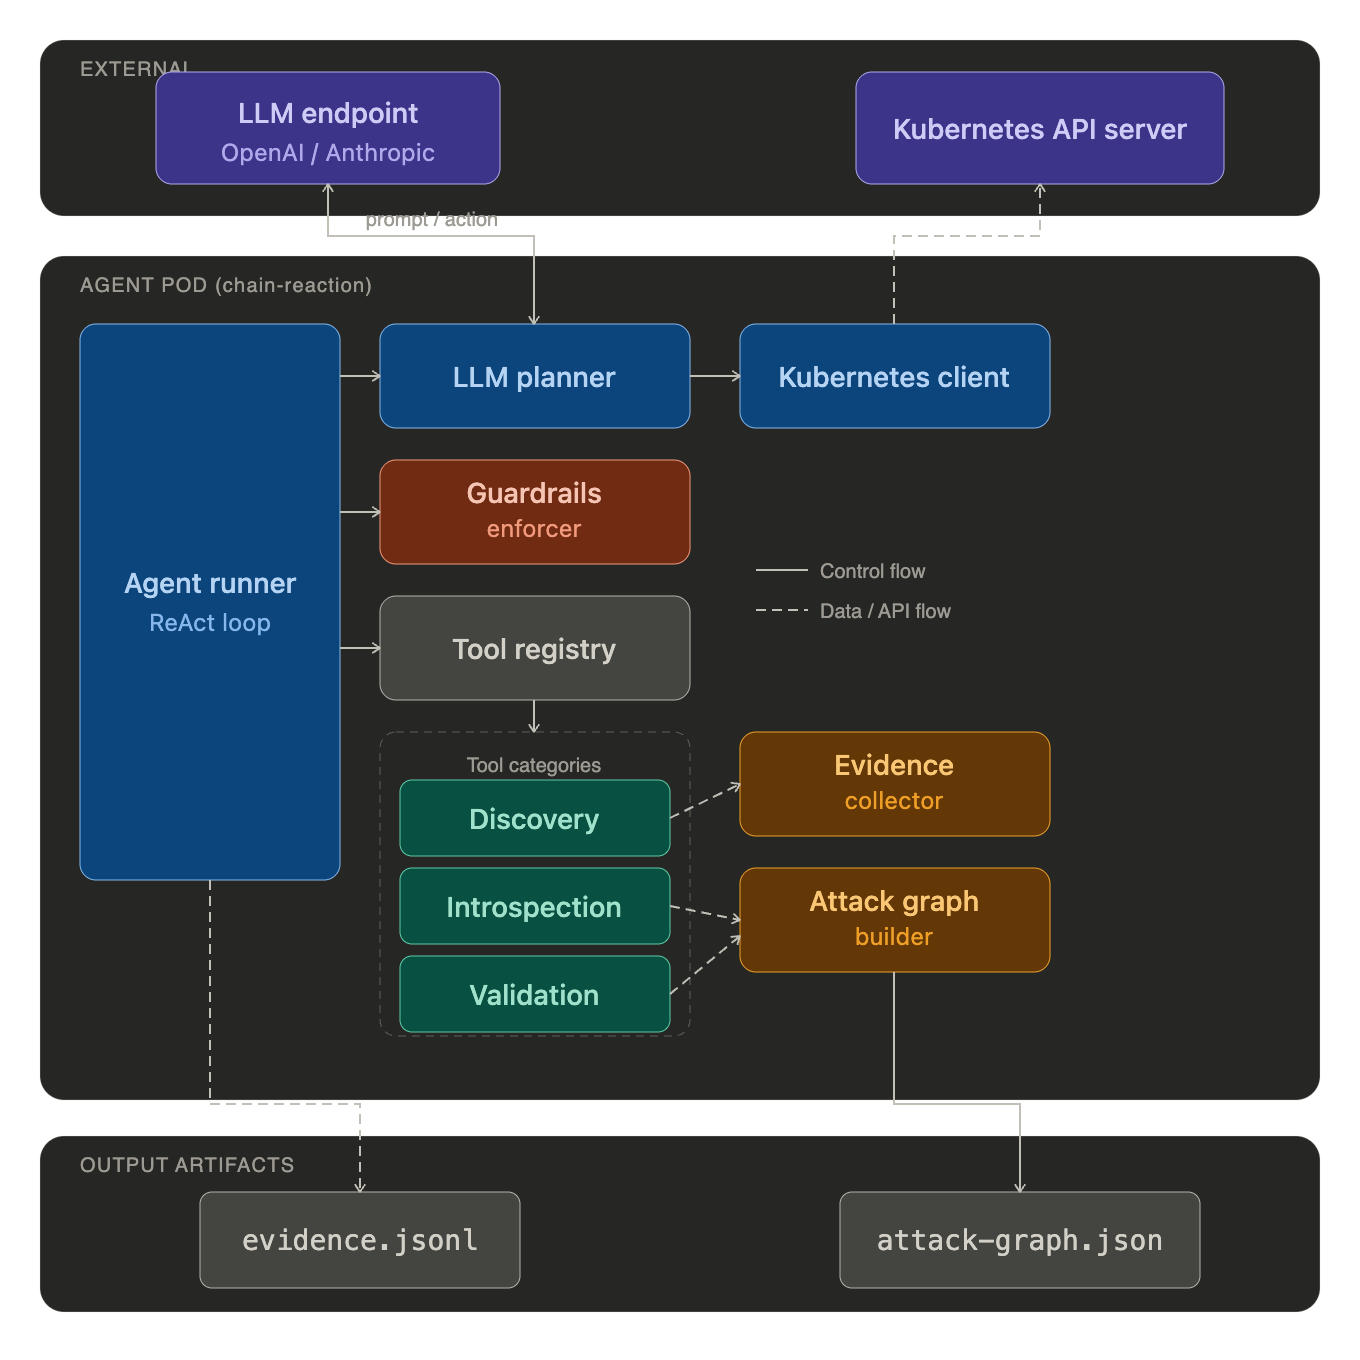
\includegraphics[width=0.85\textwidth]{architecture.png}
\caption{High-level architecture of the Chain Reaction agent. The agent pod contains six modules: the Agent Runner orchestrates the ReAct loop, the LLM Planner suggests actions, the Guardrails Enforcer validates them, the Tool Registry dispatches tool calls through the Kubernetes Client, and the Evidence Collector and Attack Graph Builder capture outputs. Solid arrows show control flow; dashed arrows show data flow.}
\label{fig:arch}
\end{figure*}

\subsection{System Components}

Table \ref{tab:components} provides a compact component summary; the subsections below expand each component's role and interfaces.

\begin{table*}[t!]
\centering
\caption{Component summary: responsibilities and primary interfaces.}
\label{tab:components}
\scriptsize
\setlength{\tabcolsep}{6pt}
\renewcommand{\arraystretch}{1.2}
\begin{tabularx}{\textwidth}{l X X}
\toprule
\textbf{Component} & \textbf{Primary responsibility} & \textbf{Inputs / outputs} \\
\midrule
Agent Runner & Orchestrates the ReAct loop, termination conditions, and run lifecycle & Inputs: run config, tool registry, planner actions; outputs: tool invocations, evidence events, graph updates \\
LLM Planner & Produces the next bounded action from current state and tool schemas & Inputs: serialized state, tool list/schemas; outputs: structured tool call (name + parameters) \\
Tool Registry & Dispatches tool calls and normalizes tool outputs & Inputs: tool name + typed parameters; outputs: typed tool results (observation payloads) \\
Guardrails Enforcer & Applies allow-lists, rate limits, time budgets, and stop conditions & Inputs: proposed action + run state; outputs: allow/deny with reason; emits guardrail events \\
Evidence Collector & Captures auditable artifacts for every executed step & Inputs: tool outputs, API responses, planner decisions; outputs: hash-chained JSONL + raw evidence files \\
Attack Graph Builder & Builds phase-annotated graphs with validated/theoretical/failed transitions & Inputs: discovered objects + step outcomes; outputs: serialized graph artifact with evidence references \\
\bottomrule
\end{tabularx}
\end{table*}

\textbf{Agent Runner.}
The Agent Runner is the central orchestrator. It implements a ReAct (Reasoning + Acting) loop: on each iteration it passes the current execution state to the LLM Planner, receives a suggested tool call, checks it against the Guardrails Enforcer, dispatches the tool through the Tool Registry, records the result with the Evidence Collector, updates the Attack Graph Builder, and evaluates termination conditions. The loop ends when the agent issues a final answer, exceeds its time budget or iteration limit, or triggers a guardrail stop.

\textbf{LLM Planner.}
The Planner wraps an LLM inference call (currently targeting the OpenAI tool-calling API). It receives the agent's accumulated state, which includes the goal, available tools with JSON schemas, and the history of prior actions and observations, and returns a structured action containing the tool to invoke and its parameters. The Planner is stateless; all context is reconstructed from the State Manager on each call.

\textbf{Tool Registry.}
The Tool Registry holds all registered tools and dispatches calls by name. Each tool implements a common interface: \texttt{Name()}, \texttt{Description()}, and \texttt{Run(ctx, input) -> (output, error)}. Tools are grouped into three categories. \emph{Discovery tools} (11 tools) enumerate cluster objects such as namespaces, pods, services, secrets, roles, role bindings, cluster roles, service accounts, config maps, endpoints, and network policies through the Kubernetes client. \emph{Introspection tools} summarize the agent's own effective permissions by issuing \texttt{SelfSubjectRulesReview} requests. \emph{Validation tools} test specific claims, such as whether the agent can read a particular secret or reach a network endpoint.

\textbf{Guardrails Enforcer.}
The Enforcer intercepts every tool call before execution and applies three classes of constraint. A \emph{namespace allow-list} restricts operations to in-scope namespaces. A \emph{token-bucket rate limiter} enforces a per-second query-per-second (QPS) cap with burst tolerance. A \emph{time budget} halts the run after a configurable duration. Any violation is logged as a guardrail event and may terminate the run.

\textbf{Evidence Collector.}
The Collector writes a JSON Lines (JSONL) log of every significant event: tool executions, API calls, LLM decisions, guardrail triggers, and validation outcomes. Each record carries a timestamp, event type, source and target resource identifiers, a payload with raw data, and an integrity field containing a SHA-256 hash chained to the previous record. The resulting evidence bundle is the primary audit artifact.

\textbf{Attack Graph Builder.}
The Builder maintains an in-memory directed graph that grows as the agent discovers objects and validates transitions. Nodes represent Kubernetes resources or identities (pods, service accounts, secrets, roles). Edges represent relationships or attack transitions (mounts, binds-to, reads, escalates-to, reaches). Each edge carries a validation status: \emph{validated} if the agent executed the step and captured evidence, \emph{theoretical} if the step is plausible but unconfirmed, or \emph{failed} if the step was attempted and blocked. The graph is serialized to JSON on completion.

\subsection{Data Flows}

A typical agent run proceeds through three phases of data flow.

\emph{Initialization.} The CLI parses flags and environment variables into a run configuration (target namespace, time budget, output directory). It creates a Kubernetes client from in-cluster credentials or a local kubeconfig, instantiates the Guardrails Enforcer with rate-limit and allow-list parameters, opens an Evidence Collector writing to the output directory, and registers all tools in the Tool Registry. The Agent Runner receives these dependencies and starts the ReAct loop.

\emph{Iterative exploration.} On each loop iteration the Runner serializes the current state (goal, tool list, action--observation history) and sends it to the LLM Planner. The Planner returns a structured action. The Runner passes the action to the Guardrails Enforcer; if the action is denied the event is logged and the loop continues. If approved, the Runner looks up the tool in the Registry and invokes it. The tool calls the Kubernetes client, which issues one or more API requests to the cluster. The raw response is returned to the Runner, which records it through the Evidence Collector and adds or updates nodes and edges in the Attack Graph. The Runner then evaluates stop conditions (time, iteration count, goal achieved, repeated failure) before starting the next iteration.

\emph{Output.} When the loop terminates, the Runner exports two artifacts: an \texttt{attack-graph.json} file containing the full node--edge graph with validation statuses and evidence references, and an \texttt{evidence.jsonl} file containing the complete, hash-chained event log. Together these artifacts allow offline review of every decision and its supporting evidence.

\section{Expected Contributions}

\subsection{Conceptual contribution}
This work frames the assumed-breach Pod position as a practical validation paradigm for cloud-native defense. Rather than treating reachability as a property derived purely from configuration, it treats exploitability as something that must be demonstrated from a real in-cluster identity under runtime constraints.

\subsection{Methodological contribution}
The project applies an LLM-guided ReAct loop to Kubernetes-native attack chain validation. It pairs adaptive tool selection with explicit guardrails (allow-lists, rate limits, time budgets, and stop conditions) to keep execution bounded and to treat the LLM as untrusted input.

\subsection{Architectural contribution}
Chain Reaction contributes a six-module agent design (Agent Runner, LLM Planner, Tool Registry, Guardrails Enforcer, Evidence Collector, Attack Graph Builder) and an evidence-first output format. The evidence layer uses a hash-chained JSONL log plus an attack graph artifact that annotates edges as validated, theoretical, or failed with evidence references.

\subsection{Applied contribution}
The work proposes a reproducible evaluation methodology against Kubernetes Goat that quantifies the gap between theoretical attack paths and runtime-confirmed chains. This yields a defender-oriented signal of how much static analysis may overestimate practical risk under real runtime controls.

\section{Project Plan and Timeline}

\subsection{Phases}
The implementation phase is structured into four phases: (1) environment and baseline setup, (2) agent architecture and tool implementation, (3) chain execution and evidence collection, and (4) evaluation and analysis. These phases align the engineering work with the planned benchmark runs in Kubernetes Goat and the downstream analysis pipeline.

\subsection{Task Breakdown}
Table \ref{tab:tasks_phase1} through Table \ref{tab:tasks_phase4} summarize the implementation tasks (T1--T20), their planned dates, dependencies, 

\begin{table*}[t!]
\centering
\caption{Phase 1 tasks (Design and Environment): task breakdown and dependencies.}
\label{tab:tasks_phase1}
\scriptsize
\setlength{\tabcolsep}{5pt}
\renewcommand{\arraystretch}{1.2}
\begin{tabularx}{\textwidth}{l X l c l l l}
\toprule
\textbf{ID} & \textbf{Task} & \textbf{Start} & \textbf{Dur (d)} & \textbf{End} & \textbf{Deps} \\
\midrule
T1 & Finalize design artifacts & 2026-04-27 & 6 & 2026-05-02 & -- & -- \\
T2 & Set up kind cluster with Kubernetes Goat & 2026-05-04 & 14 & 2026-05-18 & T1 \\
T3 & Document Kubernetes Goat scenarios & 2026-05-04 & 9 & 2026-05-14 & T1 \\
T4 & Export static/theoretical baseline catalog & 2026-05-14 & 6 & 2026-05-21 & T3 \\
T5 & Validate and finalize baseline contracts & 2026-05-18 & 7 & 2026-05-26 & T1 \\
\bottomrule
\end{tabularx}
\end{table*}

\begin{table*}[t!]
\centering
\caption{Phase 2 tasks (Agent Implementation): task breakdown and dependencies.}
\label{tab:tasks_phase2}
\scriptsize
\setlength{\tabcolsep}{5pt}
\renewcommand{\arraystretch}{1.2}
\begin{tabularx}{\textwidth}{l X l c l l l}
\toprule
\textbf{ID} & \textbf{Task} & \textbf{Start} & \textbf{Dur (d)} & \textbf{End} & \textbf{Deps} \\
\midrule
T6 & Wire live ReAct planner loop to tool registry & 2026-05-26 & 11 & 2026-06-08 & T5 \\
T7 & Activate dormant validation state and termination logic & 2026-06-01 & 20 & 2026-06-26 & T6 \\
T8 & Wire action contracts and provider-aware prompts & 2026-06-01 & 9 & 2026-06-12 & T6 \\
T9 & Extend validation and introspection tools & 2026-06-08 & 6 & 2026-06-15 & T6 \\
T10 & Upgrade graph semantics & 2026-06-08 & 6 & 2026-06-15 & T6 \\
T11 & Extend metric emission and usage tracking & 2026-06-15 & 6 & 2026-06-22 & T10 \\
T12 & Harden provider adapters and extend coverage & 2026-06-15 & 9 & 2026-06-26 & T6, T9 \\
\bottomrule
\end{tabularx}
\end{table*}

\begin{table*}[t!]
\centering
\caption{Phase 3 tasks (Integration and Evaluation): task breakdown and dependencies.}
\label{tab:tasks_phase3}
\scriptsize
\setlength{\tabcolsep}{5pt}
\renewcommand{\arraystretch}{1.2}
\begin{tabularx}{\textwidth}{l X l c l l l}
\toprule
\textbf{ID} & \textbf{Task} & \textbf{Start} & \textbf{Dur (d)} & \textbf{End} & \textbf{Deps} \\
\midrule
T13 & End-to-end integration and regression tests & 2026-06-22 & 13 & 2026-07-08 & T7, T8, T11, T12 \\
T14 & Build evaluation harness & 2026-06-15 & 20 & 2026-07-10 & T4, T11 \\
T15 & Execute scenario validation runs & 2026-07-08 & 20 & 2026-08-04 & T13, T14 \\
T16 & Debug failed or incomplete scenario runs & 2026-07-27 & 15 & 2026-08-14 & T15 \\
\bottomrule
\end{tabularx}
\end{table*}

\begin{table*}[t!]
\centering
\caption{Phase 4 tasks (Analysis and Thesis): task breakdown and dependencies.}
\label{tab:tasks_phase4}
\scriptsize
\setlength{\tabcolsep}{5pt}
\renewcommand{\arraystretch}{1.2}
\begin{tabularx}{\textwidth}{l X l c l l l}
\toprule
\textbf{ID} & \textbf{Task} & \textbf{Start} & \textbf{Dur (d)} & \textbf{End} & \textbf{Deps} \\
\midrule
T17 & Compute and analyze metrics & 2026-08-03 & 17 & 2026-08-25 & T15, T16 \\
T18 & Draft thesis chapters & 2026-08-17 & 20 & 2026-09-11 & T17 \\
T19 & Prepare demo artifacts and presentation & 2026-09-07 & 14 & 2026-09-25 & T17, T18 \\
T20 & Final review, polish, and submission & 2026-09-21 & 8 & 2026-09-30 & T19 \\
\bottomrule
\end{tabularx}
\end{table*}

\subsection{Milestones}
Table \ref{tab:milestones} summarizes the planned milestones for the FSCT 8622 implementation phase.

\begin{table*}[t!]
\centering
\caption{Chain Reaction implementation milestones (April--September 2026).}
\label{tab:milestones}
\scriptsize
\setlength{\tabcolsep}{6pt}
\renewcommand{\arraystretch}{1.2}
\begin{tabularx}{\textwidth}{l l l X}
\toprule
\textbf{ID} & \textbf{Milestone} & \textbf{Target Date} & \textbf{Completing Tasks} \\
\midrule
M1 & Design Finalization & 2026-05-02 & T1 \\
M2 & Environment and Baseline Setup & 2026-05-26 & T2--T5 \\
M3 & Planner Integration & 2026-06-08 & T6 \\
M4 & Feature Implementation & 2026-06-26 & T7--T12 \\
M5 & Testing and Evaluation & 2026-08-14 & T13--T16 \\
M6 & Analysis and Thesis Draft & 2026-09-11 & T17--T18 \\
M7 & Final Presentation and Submission & 2026-09-30 & T19--T20 \\
\bottomrule
\end{tabularx}
\end{table*}

\noindent Tasks in Table \ref{tab:milestones} and Figure \ref{fig:gantt} are labeled T1--T20 to keep the timeline readable. Table \ref{tab:tasks} provides the task legend.

\begin{table*}[t!]
\centering
\caption{Task legend for implementation timeline (T1--T20).}
\label{tab:tasks}
\scriptsize
\setlength{\tabcolsep}{6pt}
\renewcommand{\arraystretch}{1.2}
\begin{tabularx}{\textwidth}{l X}
\toprule
\textbf{ID} & \textbf{Task} \\
\midrule
T1 & Finalize design artifacts \\
T2 & Set up kind cluster with Kubernetes Goat \\
T3 & Document Kubernetes Goat scenarios \\
T4 & Export static/theoretical baseline catalog \\
T5 & Validate and finalize baseline contracts \\
T6 & Wire live ReAct planner loop to tool registry \\
T7 & Activate dormant validation state and termination logic \\
T8 & Wire action contracts and provider-aware prompts \\
T9 & Extend validation and introspection tools \\
T10 & Upgrade graph semantics \\
T11 & Extend metric emission and usage tracking \\
T12 & Harden provider adapters and extend coverage \\
T13 & End-to-end integration and regression tests \\
T14 & Build evaluation harness \\
T15 & Execute scenario validation runs \\
T16 & Debug failed or incomplete scenario runs \\
T17 & Compute and analyze metrics \\
T18 & Draft thesis chapters \\
T19 & Prepare demo artifacts and presentation \\
T20 & Final review, polish, and submission \\
\bottomrule
\end{tabularx}
\end{table*}

\subsection{Implementation Timeline}
Figure \ref{fig:gantt} shows the planned implementation timeline.

\begin{figure*}[t!]
\centering
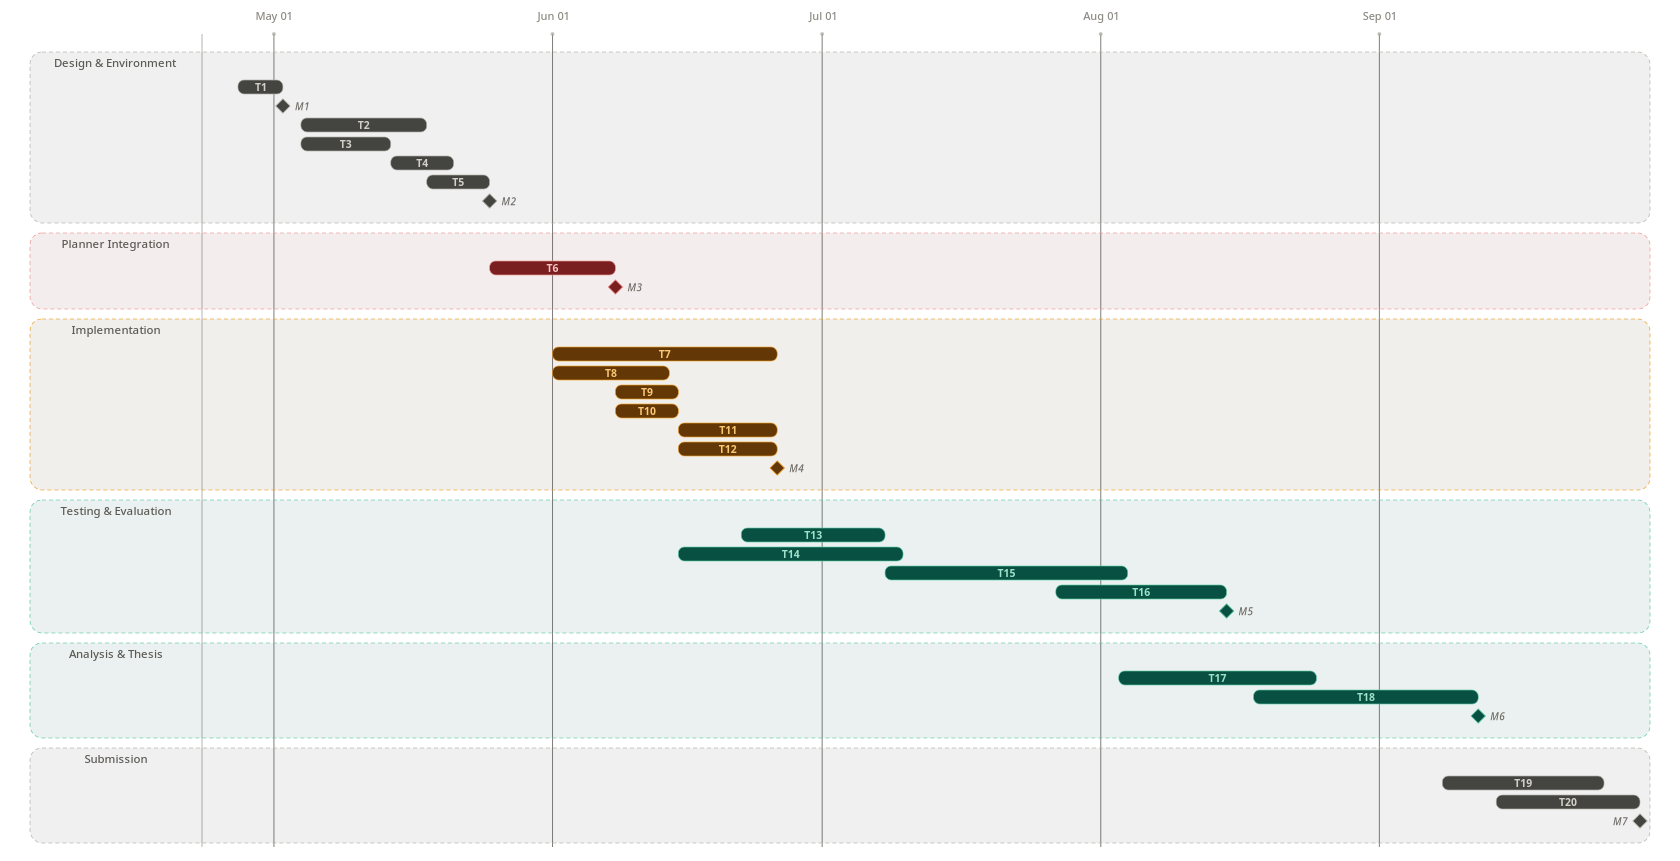
\includegraphics[width=0.95\textwidth]{gantt.png}
\caption{Chain Reaction --- Implementation Timeline (April--September 2026).}
\label{fig:gantt}
\end{figure*}

\subsection{Resource Requirements}
Table \ref{tab:resources} summarizes the primary resources required to implement and evaluate Chain Reaction in FSCT 8622.

\begin{table*}[t!]
\centering
\caption{Resource requirements for implementation and evaluation.}
\label{tab:resources}
\scriptsize
\setlength{\tabcolsep}{6pt}
\renewcommand{\arraystretch}{1.2}
\begin{tabularx}{\textwidth}{l l X}
\toprule
\textbf{Resource} & \textbf{Example} & \textbf{Use in project} \\
\midrule
Implementation language & Go + \texttt{client-go} & In-Pod agent implementation; Kubernetes API discovery, access reviews, and validations \\
Local cluster runtime & \texttt{kind} & Reproducible local clusters for repeated scenario runs and artifact collection \\
Benchmark environment & Kubernetes Goat & Controlled scenario suite (KG families) used to define baselines and measure runtime validation gap \\
Analysis stack & Python (\texttt{pandas}, \texttt{scipy.stats}, plotting) & Metric aggregation, hypothesis tests, visualization, and comparison reporting \\
External LLM endpoint & OpenAI-compatible API (configurable) & Planner inference for tool selection and step-by-step chain execution under guardrails \\
\bottomrule
\end{tabularx}
\end{table*}

Implementation uses Go and the Kubernetes \texttt{client-go} library on a local \texttt{kind} cluster running Kubernetes Goat. The evaluation and analysis pipeline is implemented in the same repository: \texttt{analyze} and \texttt{compare} compute SC, catalog-step coverage, TTC, Wilcoxon, and Spearman statistics and emit SVG/HTML reports. LLM inference is performed through an external API via a configurable provider interface.

\section{Results}

The statistics below report the recorded evaluation batches using sample mean, sample SD, CV, and a one-sample Wilcoxon signed-rank test against the paper target $\mathrm{SC}=0.80$.

\subsection{Scenario Coverage Across Batches}

Table~\ref{tab:sc_batches} reports scenario coverage for four successive five-run batches on Kubernetes Goat families KG-001 through KG-005. The planner was \texttt{react\_llm} with \texttt{openai/gpt-5.4-mini}, \texttt{--max-steps 20}, and a five-minute time budget.

\begin{table}[t]
\centering
\caption{Scenario coverage (SC) for recorded five-run batches. CV is the sample coefficient of variation (\%).}
\label{tab:sc_batches}
\scriptsize
\begin{tabular}{lccc}
\toprule
\textbf{Batch} & \textbf{SC series} & \textbf{Mean} & \textbf{CV (\%)} \\
\midrule
Initial pinned live (2026-04-09) & 0.80, 1.00, 1.00, 0.80, 0.80 & 0.88 & 12.45 \\
Post KG-004 probe fix (2026-04-10) & 0.80, 1.00, 1.00, 1.00, 1.00 & 0.96 & 9.32 \\
Post-fix closeout (2026-04-10) & 0.80, 1.00, 1.00, 1.00, 1.00 & 0.96 & 9.32 \\
KG-005 guard verify (2026-04-11) & 1.00, 1.00, 1.00, 1.00, 1.00 & 1.00 & 0.00 \\
\bottomrule
\end{tabular}
\end{table}

The paper target was $\mathrm{SC}\geq 0.80$. Every recorded run in every batch met that threshold. Mean coverage improved as two concrete failure modes were removed: a mis-typed HTTP probe against a Redis cache Service (KG-004) and an early planner final-answer that skipped the foreign-namespace proof required by KG-005-S3. Corresponding SVG figures for the final batch are included under \texttt{docs/paper/figures/}.

\subsection{Per-Family Reliability}

Table~\ref{tab:family_rel} shows per-family chain reliability (runs in which every catalog step of the family validated). On the final guard-verify batch, all five families validated in 5/5 runs.

\begin{table}[t]
\centering
\caption{Per-family chain reliability (validated / attempted runs).}
\label{tab:family_rel}
\scriptsize
\begin{tabular}{lcccc}
\toprule
\textbf{Family} & \textbf{Initial} & \textbf{Probe fix} & \textbf{Post-fix} & \textbf{Guard verify} \\
\midrule
KG-001 & 5/5 & 5/5 & 5/5 & 5/5 \\
KG-002 & 5/5 & 5/5 & 5/5 & 5/5 \\
KG-003 & 5/5 & 5/5 & 5/5 & 5/5 \\
KG-004 & 2/5 & 4/5 & 5/5 & 5/5 \\
KG-005 & 5/5 & 5/5 & 4/5 & 5/5 \\
\bottomrule
\end{tabular}
\end{table}

The moving miss is the main empirical result. After the KG-004 probe was corrected, the remaining uncovered run in the post-fix batch failed KG-005-S3: the planner stopped after two KG-004 network probes without a foreign-namespace API or Secret validation step, even though its final answer claimed full coverage. The subsequent early-stop guard refused a final answer until that evidence existed. The old miss did not recur.

\subsection{Wilcoxon Test Against the 0.80 Target}

The one-sample Wilcoxon signed-rank test compares median SC to 0.80. On the final batch every observation is 1.00, so all five signed ranks are positive. Exact two-sided enumeration at $n=5$ yields $p=0.0625$. That is the smallest two-sided exact $p$-value available at this sample size, and it is not below $\alpha=0.05$. Descriptive coverage therefore exceeds the target, but the inferential test is underpowered at five runs.

\subsection{Theory versus Scan versus Runtime}

The theoretical baseline enumerates catalog steps as defined. The deterministic \texttt{scan} baseline observes in-cluster objects but does not execute multi-step proof actions. Runtime \texttt{validate} is the only path that can label a step \texttt{validated}. Comparison artifacts (\texttt{compare --plots --tables}) therefore show a systematic gap: theory defines the chain, scan may observe supporting objects, and only the ReAct loop confirms or blocks each step with a typed failure reason. That is the answer to RQ2: a non-zero fraction of theoretically modeled steps remain unconfirmed until a bounded in-Pod proof runs, and some remain blocked even after they look reachable.

\section{Discussion}

RQ1 is answered affirmatively by the existence of fully validated multi-step chains from an assumed-breach Pod, each linked to snapshots and a JSONL evidence log. The planner selected among permission checks, secret reads, token review, and network probes without node access or privileged containers.

RQ2 is answered by the batch series. Theoretical and discovery baselines over-approximate: they cannot distinguish a Redis port that will refuse HTTP from a Service that is reachable, or a foreign-namespace object that is listed from one that the current ServiceAccount can actually get. Runtime validation collapsed those gaps when the planner chose the right proof, and documented them when it did not.

RQ3 is only partly measured. Guardrails (namespace allow-lists, QPS, time budget, max steps, and the KG-005 evidence gate) bound every run. The recorded batches used the default profile rather than a full strict/default/relaxed ablation, so the coverage--safety tradeoff is observed qualitatively: the early-stop guard reduced false ``full coverage'' claims without reducing final-batch SC.

The honest statistical reading is that $n=5$ is enough to describe stability (CV falling from 12.45\% to 0.00\%) but not enough for a two-sided exact Wilcoxon to reject 0.80 at 5\%. Larger $N$ or a one-sided test would be required to claim inferential significance.

\section{Limitations}

Kubernetes Goat on a single-node kind cluster is a lab fixture. Results do not generalize to multi-tenant production control planes, service meshes, or admission policies that were not in scope. Only five of 22 upstream Goat scenarios are in the v1 catalog; KG-006 and container-escape or node-pivot families are out of scope.

The LLM planner is a source of residual variance. One final-batch run still terminated on \texttt{max\_iterations\_reached} after already covering all families. Catalog-step coverage and TTC were not frozen for every historical batch at the same contract version, so this paper reports SC and family reliability---the quantities that were recorded for every batch---and does not invent missing TTC series.

The Wilcoxon implementation uses exact enumeration for $n<10$. With five identical positive differences the two-sided exact $p$-value cannot fall below 0.0625. That is a property of the test and the sample size, not a contradiction of the descriptive mean.

\section{Ethics and Responsible Use}

Chain Reaction assumes an authorized lab or defensive validation engagement. It does not exploit nodes, require privileged containers, emit raw ServiceAccount tokens, or bypass its own guardrails. Secret and token tools record metadata and validation outcomes only. Operators must not run the agent against clusters they do not own or lack written permission to test. The evidence bundle is designed for audit, not for credential theft.

\section{Conclusion and Future Work}

\subsection{Conclusion}
Kubernetes attack graphs and posture scanners routinely produce plausible chains but rarely provide evidence that a chain is executable from an in-cluster foothold under runtime constraints. This leaves defenders with many possible paths and limited verification that a given chain can be replayed or audited.

Chain Reaction addresses this gap by running as an assumed-breach Pod and validating chains step-by-step using bounded Kubernetes-native probes and API interactions. The architecture combines an LLM-guided ReAct planner with first-class guardrails and an evidence pipeline that produces a validated/theoretical/failed attack graph linked to a replayable evidence bundle.

Evaluation on Kubernetes Goat showed that runtime validation is both feasible and informative. Mean scenario coverage reached 1.00 (CV 0.00\%) on the final five-run guard-verify batch, with 5/5 reliability for KG-001 through KG-005. Earlier batches exposed two real blockers---a wrong KG-004 probe type and a premature KG-005 final answer---that static baselines cannot see. The Wilcoxon test at $n=5$ remains non-significant ($p=0.0625$), which we report as a sample-size limit rather than as a coverage failure.

\subsection{Future Work}
Future work can expand the scenario coverage beyond KG-001 through KG-005 to additional Kubernetes Goat families and broader cloud-native chains (for example, container escapes, node pivots, cloud metadata abuse, and admission-controller weaknesses). A second direction is a hybrid in-loop coverage gate that feeds a family-satisfaction signal back into the planner so exploration effort is directed toward unsatisfied families rather than computed post-hoc. Finally, multi-provider evaluation can compare coverage, stability, and cost trade-offs across different LLM endpoints and configurations.

\bibliographystyle{IEEEtran}
\bibliography{refs}

\end{document}
